\noindent
\begin{minipage}[t]{0.485\textwidth}
  \vspace{0pt}
  \textbf{35.} (a) Tìm hệ số góc của tiếp tuyến với đường cong $y = 9 - 2x^2$ tại điểm $(2, 1)$.\par
  \phantom{\textbf{35.}} (b) Tìm phương trình của tiếp tuyến này.

  \vspace{1pt}
  \textbf{36.} Tìm các phương trình tiếp tuyến với đường cong
  \[
  y = \frac{2}{1 - 3x}
  \]
  tại các điểm có hoành độ $0$ và $-1$.

  \vspace{1pt}
  \textbf{37.} Độ dịch chuyển (tính bằng mét) của một vật chuyển động trên một đường thẳng được cho bởi $s = 1 + 2t + \frac{1}{4}t^2$, trong đó $t$ được đo bằng giây.\par
  (a) Tìm vận tốc trung bình trong mỗi khoảng thời gian sau:\par
  \quad (i) $[1, 3]$ \quad (ii) $[1, 2]$ \quad (iii) $[1, 1.5]$ \quad (iv) $[1, 1.1]$\par
  (b) Tìm vận tốc tức thời khi $t = 1$.

  \vspace{1pt}
  \textbf{38.} Theo Định luật Boyle, nếu nhiệt độ của một khối khí giam kín được giữ cố định thì tích của áp suất $P$ và thể tích $V$ là một hằng số. Giả sử đối với một chất khí nhất định, $PV = 800$, trong đó $P$ được đo bằng pound trên inch vuông ($\text{lb/in}^2$) và $V$ được đo bằng inch khối ($\text{in}^3$).\par
  (a) Tìm tốc độ thay đổi trung bình của $P$ khi $V$ tăng từ $200\text{ in}^3$ lên $250\text{ in}^3$.\par
  (b) Biểu diễn $V$ theo hàm số của $P$ và chứng minh rằng tốc độ thay đổi tức thời của $V$ theo $P$ tỉ lệ nghịch với bình phương của $P$.

  \vspace{1pt}
  \textbf{39.} (a) Dùng định nghĩa đạo hàm để tìm $f'(2)$, với $f(x) = x^3 - 2x$.\par
  \phantom{\textbf{39.}} (b) Tìm phương trình tiếp tuyến với đường cong $y = x^3 - 2x$ tại điểm $(2, 4)$.\par
  \makebox[0pt][r]{\graphicon\hspace{3pt}}(c) Minh họa câu (b) bằng cách vẽ đường cong và tiếp tuyến trên cùng một màn hình đồ thị.

  \vspace{1pt}
  \textbf{40.} Tìm một hàm số $f$ và một số $a$ sao cho
  \[
  \lim_{h \to 0} \frac{(2 + h)^6 - 64}{h} = f'(a)
  \]

  \vspace{1pt}
  \textbf{41.} Tổng chi phí để trả một khoản vay sinh viên với lãi suất $r\%$ mỗi năm là $C = f(r)$.\par
  (a) Đạo hàm $f'(r)$ có ý nghĩa gì? Đơn vị của nó là gì?\par
  (b) Khẳng định $f'(10) = 1200$ có ý nghĩa gì?\par
  (c) Đạo hàm $f'(r)$ luôn dương hay nó có đổi dấu?

  \vspace{4pt}
  \noindent{\color{stewartcyan}\textbf{42--44}}\quad Đồ lại hoặc sao chép đồ thị của hàm số. Sau đó phác thảo đồ thị đạo hàm của nó ngay phía dưới.

  \vspace{3pt}
  \noindent
  \begin{minipage}[t]{0.48\linewidth}
    \textbf{42.}\par\vspace{1pt}
    \centering
    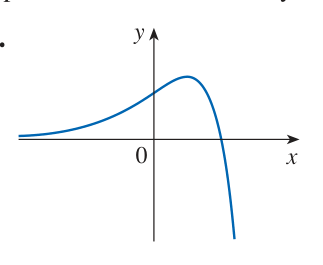
\includegraphics[width=0.95\linewidth]{images/p0204_fig4.png}
  \end{minipage}\hfill
  \begin{minipage}[t]{0.48\linewidth}
    \textbf{43.}\par\vspace{1pt}
    \centering
    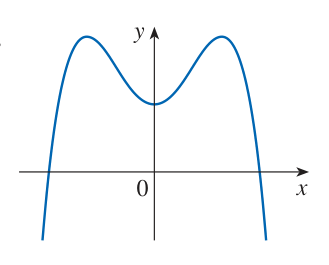
\includegraphics[width=0.95\linewidth]{images/p0204_fig5.png}
  \end{minipage}
\end{minipage}%
\hfill
\begin{minipage}[t]{0.485\textwidth}
  \vspace{0pt}
  \noindent\textbf{44.}\par\vspace{1pt}
  \centering
  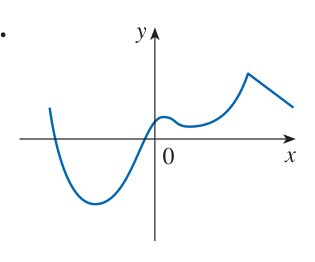
\includegraphics[width=0.68\linewidth]{images/p0204_fig1.png}

  \vspace{3pt}
  {\color{stewartcyan}\rule{\linewidth}{0.6pt}}
  \vspace{2pt}

  \raggedright
  \noindent{\color{stewartcyan}\textbf{45--46}}\quad Tìm đạo hàm của $f$ bằng cách sử dụng định nghĩa đạo hàm. Tập xác định của $f'$ là gì?\par
  \vspace{2pt}
  \noindent
  \begin{minipage}[t]{0.48\linewidth}
    \textbf{45.} $f(x) = \dfrac{2}{x^2}$
  \end{minipage}\hfill
  \begin{minipage}[t]{0.48\linewidth}
    \textbf{46.} $f(t) = \dfrac{1}{\sqrt{t + 1}}$
  \end{minipage}

  \vspace{2pt}
  {\color{stewartcyan}\rule{\linewidth}{0.6pt}}
  \vspace{2pt}

  \noindent\textbf{47.} (a) Nếu $f(x) = \sqrt{3 - 5x}$, hãy dùng định nghĩa đạo hàm để tìm $f'(x)$.\par
  \phantom{\textbf{47.}} (b) Tìm tập xác định của $f$ và $f'$.\par
  \makebox[0pt][r]{\graphicon\hspace{3pt}}(c) Vẽ đồ thị của $f$ và $f'$ trên cùng một màn hình. So sánh các đồ thị để xem câu trả lời của bạn ở phần (a) có hợp lý hay không.

  \vspace{2pt}
  \noindent\textbf{48.} (a) Tìm các đường tiệm cận của đồ thị hàm số
  \[
  f(x) = \frac{4 - x}{3 + x}
  \]
  và sử dụng chúng để phác thảo đồ thị.\par
  \phantom{\textbf{48.}} (b) Dùng đồ thị ở phần (a) để phác thảo đồ thị của $f'$.\par
  \phantom{\textbf{48.}} (c) Dùng định nghĩa đạo hàm để tìm $f'(x)$.\par
  \makebox[0pt][r]{\graphicon\hspace{3pt}}(d) Vẽ đồ thị của $f'$ và so sánh với hình phác thảo của bạn ở phần (b).

  \vspace{2pt}
  \noindent\textbf{49.} Cho đồ thị của $f$ như hình vẽ. Hãy chỉ ra các điểm mà tại đó $f$ không có đạo hàm và nêu rõ lý do.\par\vspace{1pt}
  \centering
  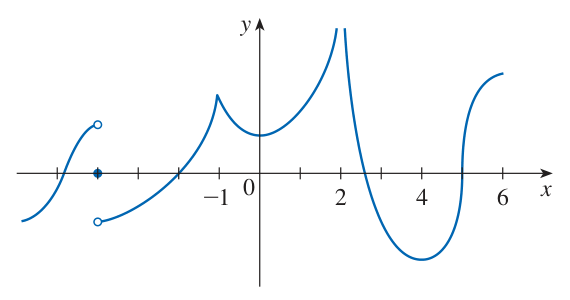
\includegraphics[width=0.74\linewidth]{images/p0204_fig2.png}

  \vspace{3pt}
  \raggedright
  \noindent\textbf{50.} Hình vẽ hiển thị đồ thị của $f$, $f'$ và $f''$. Hãy xác định từng đường cong và giải thích sự lựa chọn của bạn.\par\vspace{1pt}
  \centering
  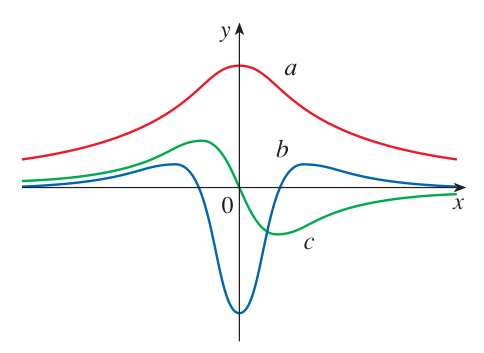
\includegraphics[width=0.74\linewidth]{images/p0204_fig3.png}
\end{minipage}

\vfill
\begin{center}
  \scriptsize\color{stewartgray}
  Bản quyền thuộc Cengage Learning. Bản dịch tiếng Việt phục vụ mục đích học tập và nghiên cứu.
\end{center}
